\documentclass[lang=cn]{elegantpaper}

\title{Mealy状态机}

\begin{document}

\maketitle



本题中输出需要由状态决定和当前输入,因此需要设定不同的状态跳转方式和在特定输入的情况下的输出。对于输出来说,需要在不同的状态跳变时一同变化,因此使用 \lstinline{<=} 进行赋值。


 \section{状态机运行模式}

转换图如 \figref{01} 。

\begin{figure}[htb]
    \centering
    \caption{转换图}\label{01}
    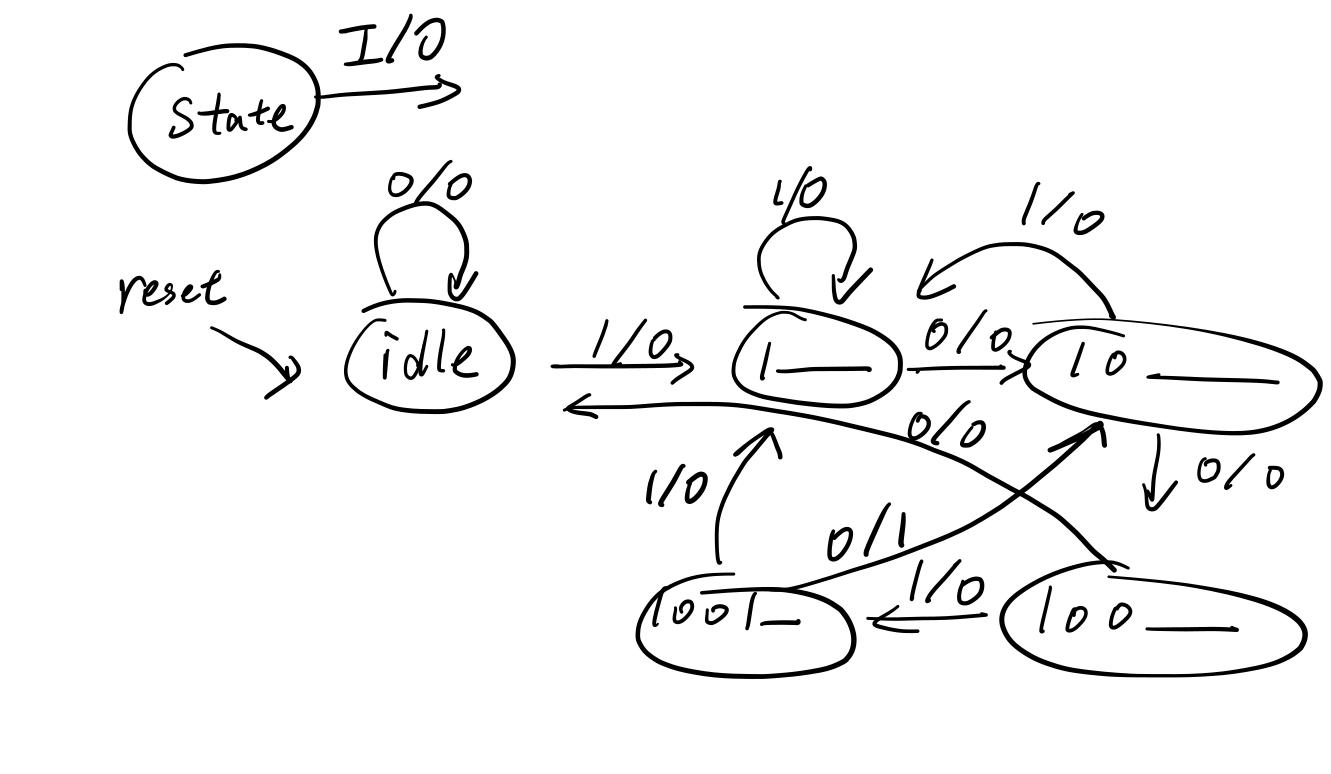
\includegraphics[width=0.6\textwidth]{trans.png}
\end{figure}




波形如 \figref{02} 。


\begin{figure}[htb]
    \centering
    \caption{波形图}\label{02}
    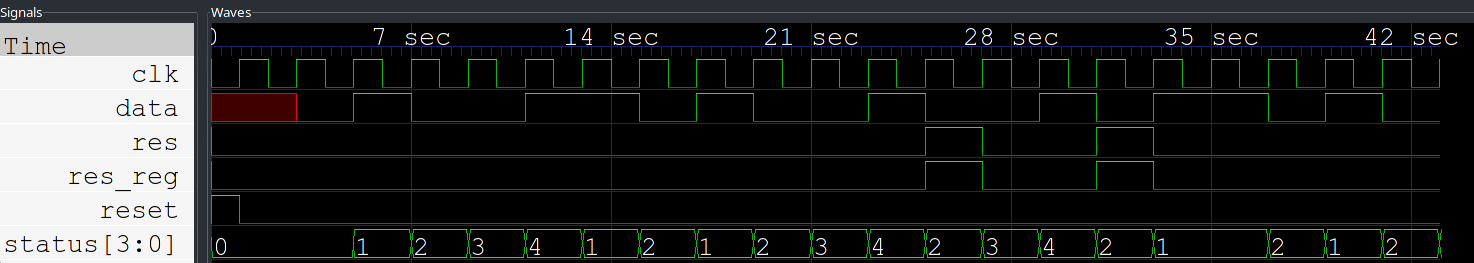
\includegraphics[width=0.6\textwidth]{wave.png}
\end{figure}


\end{document}